\chapter{Evaluation}
\label{chap:evaluation}
In diesem Kapitel wird die Umsetzung der Anwendung bewertet.
Wie \cref{fig:screen-main}, \cref{fig:screen-filter} und \cref{fig:screen-statements} zeigen, war die Umsetzung der Grundfunktion der Anwendung erfolgreich.
Die Anwendung ist unter \url{https://tools.wmflabs.org/wdumps} erreichbar.
Viele der Anforderungen wurden bereits im Design beachtet.
Zur Evaluation wird deshalb nur ein Aspekt genauer betrachtet: die Konsistenz der erzeugten Dumps.

Die umgesetzte Anwendung verwendet Wikidata-Toolkit zum Erzeugen der Dumps verwendet.
Die vollständigen RDF-Exporte von Wikidata hingegen werden von Wikibase, einer PHP-Erweiterung für MediaWiki, generiert.
Damit kann es zwischen beiden Implementierung zu Differenzen kommen.
Um diese Differenzen zu finden und zu beheben wird in diesem Kapitel ein offizielle RDF-Export von Wikidata mit den von Wikidata-Toolkit generierten RDF Daten verglichen. 

\begin{figure}
  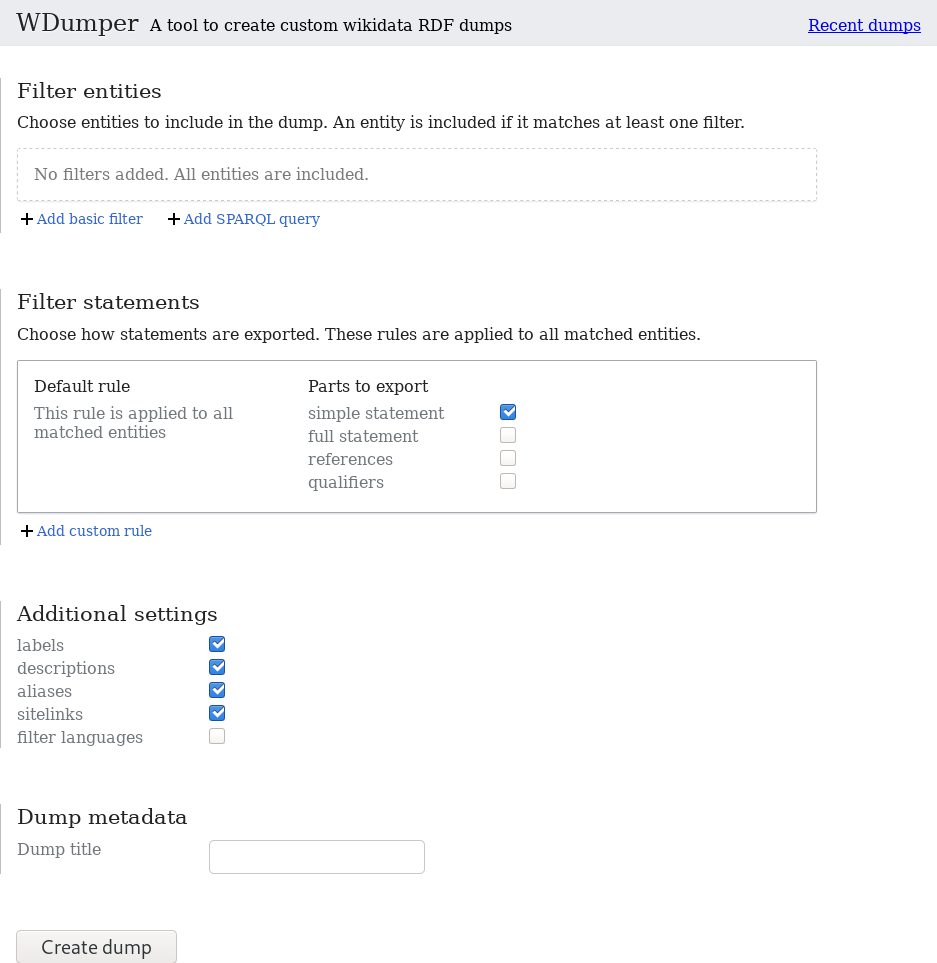
\includegraphics[width=\textwidth]{pics/screen-main}
  \caption{Startseite mit Interface zur Angabe von Filtern. In der gezeigten Standardeinstellung werden die simple Statements, Terme und Sitelinks zu jeder Entität in allen Sprachen exportiert.}
  \label{fig:screen-main}
\end{figure}

\begin{figure}
  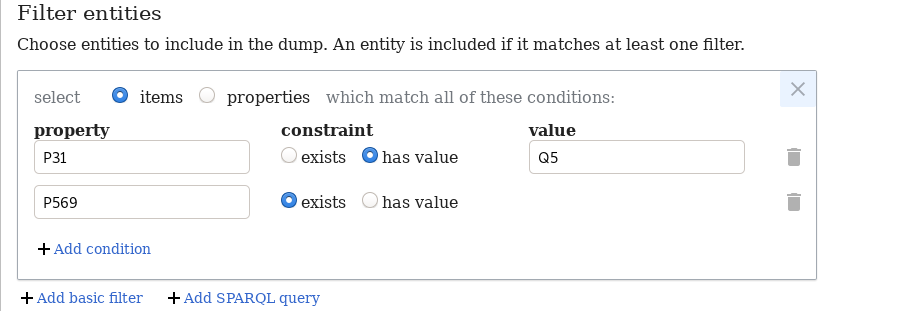
\includegraphics[width=\textwidth]{pics/screen-filter}
  \caption{Sektion zum Filtern: Im Beispiel werden nur Entities, welche Instanz von (P31) Mensch (Q5) sind und ein Statement für P569 (Geburtsdatum) besitzen exportiert.}
  \label{fig:screen-filter}
\end{figure}

\begin{figure}
  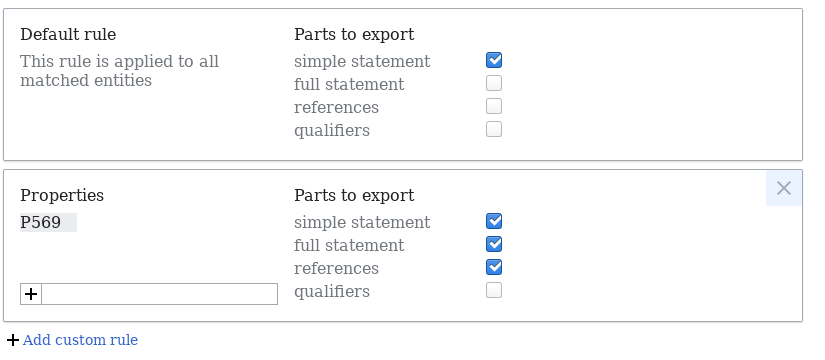
\includegraphics[width=\textwidth]{pics/screen-statements}
  \caption{Sektion mit Statementeinstellungen: es werden alle simple Statements exportiert und dazu die Statements für P569 (Geburtsdatum) mit Referenzen}
  \label{fig:screen-statements}
\end{figure}

\section{Vorgehen}
Für den Vergleich werden die JSON- und RDF-Exporte von Wikidata vom 26. August 2019 verwendet.
Die Daten und der Quellcode für den Vergleich sind über Zenodo verfügbar\cite{zenodo-diff-data}.
Da sich die Daten während der Generierung des Exports verändern, beschreiben die JSON- und RDF-Exporte nicht exakt dieselben Daten.
Deswegen werden für den Vergleich zusätzlich noch die Wikidata incremental Dumps verwendet.
Diese enthalten die JSON-Darstellung aller in einem Zeitraum geänderten Wikidata Dokumente, zusammen mit Revisionsnummer und Datum der Revision. 
Damit können Dokumente des JSON-Dumps, deren Revisionsnummer nicht identisch zu dem entsprechenden Dokument in dem RDF-Export ist, durch die aktualisierte Version ersetzt werden.
Um die Revisionsnummer eines Dokuments des RDF-Exports zu bestimmen wird das mit dem Prädikat \verb|schema:dateModified| angegebene Änderungsdatum verwendet.

Nachdem beide Exporte so auf die selbe Version gebracht wurden, wird mit der Anwendung aus dem JSON-Export RDF erzeugt.
Dazu werden keine Filter verwendet, entsprechend sollte die Anwendung in diesem Fall den RDF-Export komplett reproduzieren.
Praktisch ist dabei, dass die Dokumente sowohl in dem JSON-Export als auch in dem RDF-Export in der selben Reihenfolge gespeichert sind.
Damit kann der Vergleich für jedes Paar von Dokumenten separat erfolgen.

Ein Problem für den Vergleich stellen die Value Nodes dar.
Die IRI für Value Nodes enthält im RDF-Export von Wikidata einen Hash, der auf dem internen Datenmodell basiert und daher schwer zu reproduzieren ist.
Aus diesem Grund stimmen die von Wikidata-Toolkit generierten Tripel nicht eins-zu-eins mit denen des RDF-Exports überein, da die IRIs von Values Nodes einen anderen Hash benutzen.
Um dieses Problem zu lösen, muss zur Bestimmung der Differenzen eine Abbildung der IRIs aus dem Export zu den IRIs der generierten Daten bestimmt werden.
Die Abbildung lässt sich leicht bestimmen, da Value Nodes immer nur von Nodes mit festen IRIs referenziert werden (Referenz und Statement Nodes).
Die Value Nodes können deswegen über ihre Verbindungen zu diesen Knoten identifiziert und abgeglichen werden.
Falls die Abbildung trotzdem noch uneindeutig ist, wird anhand der Objekte der Tripel der entsprechende Value Nodes entschieden.
Diese Lösung funktioniert auch zum Abgleich der im Export vorkommenden Blank Nodes.

Nach diesem Abgleich werden die Tripel verglichen.
Die Differenzen sind die Tripel, die entweder nur im Export oder nur in dem generierten RDF vorkommen.
Einige Differenzen sind schon vorher bekannt, die bspw. aufgrund von fehlenden Funktionen in Wikidata-Toolkit entstehen.
Zur Vereinfachung der Analyse werden folgende Tripel von dem Vergleich ausgenommen:
\begin{enumerate}
\item Tripel, deren Subjekt das Prefix \verb|wdata:| besitzt. Diese Tripel gehören zu den Data Nodes, welche aktuell von Wikidata-Toolkit nicht generiert werden.
Die Data Nodes enthalten Metadaten zu dem Entity, wie \verb|schema:dateModified|.
\item Entities, welche nur im RDF-Export oder nur im JSON-Export enthalten. Dieser Fall kann aus zwei Gründen auftreten: Löschungen in der Zeit zwischen der Erstellung beider Exporte, oder Weiterleitungen.
  Die RDF-Exporte von Wikidata enthalten für jede Weiterleitung ein Tripel mit Prädikat \verb|owl:sameAs|, welche Wikidata-Toolkit nicht generiert.
\item Tripel, die normalisierte Werte für Properties angeben und die entsprechenden Value Nodes. Wikidata-Toolkit unterstützt normalisierte Werte nicht, weshalb ein Vergleich hier nicht möglich ist.
\item Tripel mit Prädikat \verb|schema:name| oder \verb|skos:prefLabel|. Diese Tripel sind Duplikate der Tripel mit Prädikat \verb|rdfs:label|, und Wikidata-Toolkit generiert aktuell nur \verb|rdfs:label|-Tripel.
\item Tripel mit den Prädikaten \verb|owl:onProperty| oder \verb|owl:complementOf| sowie Tripel mit Objekten aus dieser Liste: \verb|owl:Class|, \verb|owl:Thing|, \verb|owl:Restriction|, \verb|owl:DatatypeProperty| oder \verb|owl:ObjectProperty|. Diese Tripel werden für OWL-Definitionen der Wikidata Properties verwendet.
Im RDF-Export finden sich die Tripel in dem Dokument für die Property, Wikidata-Toolkit generiert die Tripel jedoch wenn die Property das erste Mal verwendet wird. Damit lassen sich diese Tripel nicht dokumentweise vergleichen.
\end{enumerate}

\section{Ergebnis} 

\begin{table}
  \begin{tabular}{lp{0.6\textwidth}}
    \bfseries{Stichwort} & \bfseries{Beschreibung} \\
    wdata: & Nicht implementiert \\
    normalisierte Werte & Nicht implementiert \\
    owl:sameAs & Weiterleitungen nicht implementiert \\
    \\
    Statement ID & Groß/Kleinschreibung der Item-ID in der Statement ID nicht beachtet \\
    Language Tags & Unterschiedliche Language Tags \\
    simple value (Referenz) & Bei Referenzen werden nur komplexe Werte angegeben \\
    complex value (SomeValue) & SomeValue Snaks wird auch ein BNode für den komplexen Wert generiert \\
    Sitelinks Siteinfo & bei Sitelinks fehlen Tripel für \verb|schema:name|, \verb|schema:isPartOf|, \verb|wikibase:wikiGroup| \\
    \\
    invalide IRIs & URL-Werte mit \verb|"| erzeugen invalides RDF \\
    Koordinaten & Längen- und Breitengrad in Koordinatenwerten vertauscht \\
    Dezimalzahlen & Nicht konforme Verwendung von wissenschaftlicher Darstellung \\
    Kalender & Umrechnung von Datumsangaben in gregorianischen Kalender fehlt \\
    invalide Daten & Mehrere Abweichungen bei invaliden Daten (30 Februar etc) \\
    Commons Link & Links zu Wikimedia Commons sind unterschiedlich (falsches Prefix und Behandlung von Sonderzeichen) \\
    Formeln & Konvertierung nach MathML fehlt \\
    falsche Literaltypen & \verb|xsd:int| vs \verb|xsd:integer|, Tippfehler bei \verb|wikibase:GlobeCoordinatesValue|, fehlender Datentyp \verb|wikibase:MusicalNotation| \\
    Rundung & Gleitkommazahlen unterscheiden sich aufgrund von Rundungsfehlern \\
    \\
    Datumdeduplizierung & Datumsangaben wurden falsch dedupliziert (Präzision nicht beachtet) \\
    Referenzdeduplizierung & Gleiche Referenzen mit unterschiedlicher Snak-Reihenfolge werden nicht dedupliziert \\
  \end{tabular}
  \caption{Übersicht der festgestellten Differenzen (aus Sicht von Wikidata-Toolkit)}
  \label{tab:wdtk-diff}
\end{table}

Eine Übersicht über das Ergebnis des Vergleichs gibt \cref{tab:wdtk-diff}.
Die meisten Differenzen lassen sich einfach beheben, oft sind nur wenige Veränderungen an Wikidata-Toolkit notwendig. Dazu zählen: Statement ID, Sitelinks Siteinfo, invalide IRIs, simple value (Referenz), complex value (SomeValue), Koordinaten, Dezimalzahlen, Commons Link, Formeln, falsche Literaltypen, Datumdeduplizierung und Referenzdeduplizierung.
Diese Korrekturen werden auch dem Wikidata-Toolkit Projekt beigetragen.
Ein Großteil der Differenzen treten bei komplexen Literalwerten, wie Zeitdaten oder Geokoordinaten auf.
Während die meisten Differenzen relativ harmlose Formfehler sind (wie das Verwenden falscher Literaltypen), sind auch drei inhaltliche Fehler aufgefallen.

Der erste Fall ist die Vertauschung von Längen- und Breitengrad bei Koordinatenangaben.
Statt \verb|"Point(4.6681 50.6411)"^^geo:wktLiteral| generiert Wikidata-Toolkit \verb|"Point(50.641111111111 4.6680555555556)"^^geo:wktLiteral| (die Abweichung der Fließkommazahlen liegen an dem Rundungsproblem). Entsprechend der GeoSPARQL Spezifikation\cite{spec:geosparql} ist für den Datentyp \verb|geo:wktLiteral| die Reihenfolge der Koordinaten abhängig vom angegebenen Koordinatensystem.
Für den Standardwert CRS84\footnote{\url{http://www.opengis.net/def/crs/OGC/1.3/CRS84}} ist die Reihenfolge \emph{Längengrad}-\emph{Breitengrad}, was entgegen der verbreiteten Darstellung 50°38'28"N, 4°40'5"E ist.

Der zweite Fall hängt mit der Deduplizierung von Value Nodes zusammen.
Um die Größe des Dumps zu reduzieren, werden für gleiche komplexe Werte die selben Value Nodes verwendet, sodass die Daten nicht zweimal abgespeichert werden müssen.
Wikidata-Toolkit verwendet dazu einfach den Hash, der auch in der IRI für die Value Node vorkommt.
Falls schon ein Value Node für diesen Hash generiert wurde, werden die Daten nicht erneut geschrieben.
Bei Daten und Zeitwerten berücksichtigt dieser Hash jedoch die Präzision des Wertes nicht.
Damit werden Werte, die sich nur in der Präzisionsangabe unterscheiden, zum selben Value Node.
Die Präzision aller Zeitwerte für diesen Zeitpunkt entspricht dann der Präzision des zuerst verarbeiteten Zeitwerts.
Dieser Fehler lässt sich einfach beheben, in dem auch die Präzision mit in den Hash aufgenommen wird.
Ein ähnliches Problem tritt im Zusammenhang mit Referenzen auf.
Hier wird auch die Reihenfolge der Properties vom Hash berücksichtigt, sodass Referenzen mit gleichem Inhalt aber unterschiedlicher Reihenfolge unterschiedliche Hashes erhalten.
Diese Differenz ist natürlich deutlich weniger kritisch (ob diese Differenz überhaupt einen inhaltlichen Fehler darstellt ist streitbar) lässt sich aber genauso einfach beheben.

Der dritte Fall betrifft auch Datumsangaben.
Die XML-Schema Spezifikation verlangt, dass Literale mit Typ \verb|xsd:dateTime| im proleptischen gregorianischen Kalender angegeben werden.\footnote{\url{https://www.w3.org/TR/xmlschema11-2/\#dateTime}}
Im JSON-Export sind jedoch auch Daten im julianischen Kalender vorhanden.
Wikidata-Toolkit hat die notwendige Konversion zum gregorianischen Kalender noch nicht implementiert.
Dieser Fehler kann die Daten um mehrere Tage verändern. Ein Beispiel dafür sind diesen beiden Tripel:
\begin{lstlisting}[language=SPARQL]
# tripel aus dem Wikidata RDF Export
wd:Q45 wdt:P571 "1143-10-12T00:00:00Z"^^xsd:dateTime .

# tripel von Wikidata-Toolkit generiert
wd:Q45 wdt:P571 "1143-10-05T00:00:00Z"^^xsd:dateTime .
\end{lstlisting}

Datumsangaben sind allgemein komplex, was sich auch in weiteren Differenzen zeigt. 
Diese sind zwar inhaltlich nicht falsch, entsprechen aber trotzdem nicht der Spezifikation.
Ein Beispiel sind negative Jahreszahlen.
Die XML Schema Spezifikation verlangt hier, dass die Jahreszahl (ohne das Minuszeichen) vierstellig ist.
Wikidata-Toolkit generiert aber insgesamt nur vier Stellen (mit Minuszeichen).
Weiterhin gibt es Abweichungen bei invaliden Daten.
Der RDF-Export von Wikidata versucht diese zu bereinigen.
Wenn Tag oder Monat 0 ist, wird dieser auf 1 geändert und der Tag wird auf die maximale Anzahl an Tagen für diesen Monat begrenzt.
Das wird auch von der XML-Schema Spezifikation so verlangt.
Wikidata-Toolkit verändert die Daten jedoch deutlich weniger, sodass sich die Tripel hier unterscheiden.

Weitere Differenzen finden sich bei den Language Tags.
Das Problem tritt hier bei weniger verbreiteten Sprachen auf, die teilweise keinen Language Code nach BCP47\footnote{\url{https://tools.ietf.org/html/bcp47}} besitzen.
Wikidata Toolkit versucht hier, die Wikimedia Language Codes auf BCP47 Codes abzubilden.
Diese Abbildung wird im RDF Export von Wikidata nicht vorgenommen.
In diesem Fall ist es schwer zu sagen, welche Variante "`korrekt"' ist, da RDF explizit die Verwendung von BCP47 vorsieht.
Dennoch sollte sich am Ende für eine einheitliche Variante entschieden werden.
Die Verwendung der Wikimedia Language Codes, die sich auch an BCP47 orientieren, stellt hier die einfachste Lösung da.

Insgesamt zeigt dieser Vergleich, dass das komplexe Datenmodell von Wikidata auch einige Tücken hat.
Viele der gefundenen Differenzen sind subtil und wären ohne explizites Suchen danach vermutlich schwer zu finden.
Durch die Verbesserung von Wikidata-Toolkit können diese Differenzen reduziert werden.
% 
% owl#sameAs entities missing in generated:
%     <https://www.wikidata.org/wiki/Special:EntityData/Q6825> <http://www.w3.org/1999/02/22-rdf-syntax-ns#type> <http://schema.org/Dataset> .
%     <https://www.wikidata.org/wiki/Special:EntityData/Q6825> <http://schema.org/about> <http://www.wikidata.org/entity/Q6825> .
%     <https://www.wikidata.org/wiki/Special:EntityData/Q6825> <http://schema.org/version> "942411738"^^<http://www.w3.org/2001/XMLSchema#integer> .
%     <https://www.wikidata.org/wiki/Special:EntityData/Q6825> <http://schema.org/dateModified> "2019-05-15T10:13:36Z"^^<http://www.w3.org/2001/XMLSchema#dateTime> .
%     <http://www.wikidata.org/entity/Q6825> <http://www.w3.org/2002/07/owl#sameAs> <http://www.wikidata.org/entity/Q26709563> .
% 
% IRI not correctly escaped in generated:
%     <http://www.wikidata.org/entity/Q8479> <http://www.wikidata.org/prop/direct/P94> <http://commons.wikimedia.org/wiki/File:Imperial_Monogram_of_Tsar_Peter_I_\"The_Great\"_of_Russia,_Variant_2.svg> .
% 
% In official dumps, some statement IDs are lowercase (not all though):
%     <http://www.wikidata.org/entity/Q31> <http://www.wikidata.org/prop/P349> <http://www.wikidata.org/entity/statement/Q31-C3BA4AF9-CC89-4B2D-B9ED-2211228CEF09> .
%     <http://www.wikidata.org/entity/Q31> <http://www.wikidata.org/prop/P38> <http://www.wikidata.org/entity/statement/q31-2AD587B8-A440-438E-A7E0-3F992600D36D> .
% 
% Official dumps use different coordinate order:
%     <http://www.wikidata.org/entity/Q31> <http://www.wikidata.org/prop/direct/P5140> "Point(4.6681 50.6411)"^^<http://www.opengis.net/ont/geosparql#wktLiteral> [offical]
%     <http://www.wikidata.org/entity/Q31> <http://www.wikidata.org/prop/direct/P5140> "Point(50.641111111111 4.6680555555556)"^^<http://www.opengis.net/ont/geosparql#wktLiteral>) [generated]]
% 
% Value normalization (+ normalized value, normalized reference value, normalized quantity value, normalized qualifier value):
%     <http://www.wikidata.org/entity/Q31> <http://www.wikidata.org/prop/direct/P6897> "+99"^^<http://www.w3.org/2001/XMLSchema#decimal> . [official]
%     <http://www.wikidata.org/entity/Q31> <http://www.wikidata.org/prop/direct/P6897> "99"^^<http://www.w3.org/2001/XMLSchema#decimal> . [gen]
% 
% Wrong serialization of decimals:
%     <http://www.wikidata.org/entity/Q2294> <http://www.wikidata.org/prop/direct/P2069> "0.000000000000000000000000014106067"^^<http://www.w3.org/2001/XMLSchema#decimal> .
%     <http://www.wikidata.org/entity/Q2294> <http://www.wikidata.org/prop/direct/P2200> "0.00000000000000000016021766208"^^<http://www.w3.org/2001/XMLSchema#decimal> .
%     ----
%     <http://www.wikidata.org/entity/Q2294> <http://www.wikidata.org/prop/direct/P2200> "1.6021766208E-19"^^<http://www.w3.org/2001/XMLSchema#decimal> .
%     <http://www.wikidata.org/entity/Q2294> <http://www.wikidata.org/prop/direct/P2069> "1.4106067E-26"^^<http://www.w3.org/2001/XMLSchema#decimal> .
% 
% Language tags are different:
%     <http://www.wikidata.org/entity/Q31> <http://www.w3.org/2000/01/rdf-schema#label> "Belçika"@crh .
%     <http://www.wikidata.org/entity/Q31> <http://www.w3.org/2000/01/rdf-schema#label> "Belgien"@ksh .
%     <http://www.wikidata.org/entity/Q31> <http://www.w3.org/2000/01/rdf-schema#label> "Bélgica"@cbk-zam .
%     <http://www.wikidata.org/entity/Q31> <http://www.w3.org/2000/01/rdf-schema#label> "Belgique"@nrm .
%     <http://www.wikidata.org/entity/Q31> <http://www.w3.org/2000/01/rdf-schema#label> "Bèlge"@roa-tara .
%     <http://www.wikidata.org/entity/Q31> <http://www.w3.org/2000/01/rdf-schema#label> "Belgija"@sr-el .
%     <http://www.wikidata.org/entity/Q31> <http://www.w3.org/2000/01/rdf-schema#label> "Белгија"@sr-ec .
%     <https://eml.wikipedia.org/wiki/B%C3%A9lgi> <http://schema.org/inLanguage> "egl" .
%     ---
%     <http://www.wikidata.org/entity/Q31> <http://www.w3.org/2000/01/rdf-schema#label> "Belgien"@mis-x-rip .
%     <http://www.wikidata.org/entity/Q31> <http://www.w3.org/2000/01/rdf-schema#label> "Bélgica"@cbk-x-zam .
%     <http://www.wikidata.org/entity/Q31> <http://www.w3.org/2000/01/rdf-schema#label> "Belgique"@fr-x-nrm .
%     <http://www.wikidata.org/entity/Q31> <http://www.w3.org/2000/01/rdf-schema#label> "Bèlge"@it-x-tara .
%     <http://www.wikidata.org/entity/Q31> <http://www.w3.org/2000/01/rdf-schema#label> "Belgija"@sr-Latn .
%     <http://www.wikidata.org/entity/Q31> <http://www.w3.org/2000/01/rdf-schema#label> "Белгија"@sr-Cyrl .
%     <https://eml.wikipedia.org/wiki/B%C3%A9lgi> <http://schema.org/inLanguage> "eml" .
% 
% File URIs are different:
%     <http://www.wikidata.org/entity/Q31> <http://www.wikidata.org/prop/direct/P41> <http://commons.wikimedia.org/wiki/Special:FilePath/Flag%20of%20Belgium%20%28civil%29.svg> .
%     ---
%     <http://www.wikidata.org/entity/Q31> <http://www.wikidata.org/prop/direct/P41> <http://commons.wikimedia.org/wiki/File:Flag_of_Belgium_%28civil%29.svg> .
% 
% Official dump has blank node for some-value statements:
%     <http://www.wikidata.org/entity/Q31> <http://www.wikidata.org/prop/direct/P1589> _:genid0-0-1 .
%     ---
% 
% EntityData is missing
% 
% Time value problems
%     <http://www.wikidata.org/entity/Q45> <http://www.wikidata.org/prop/direct/P571> "1143-10-12T00:00:00Z"^^<http://www.w3.org/2001/XMLSchema#dateTime> .
%     ---
%     <http://www.wikidata.org/entity/Q45> <http://www.wikidata.org/prop/direct/P571> "1143-10-05T00:00:00Z"^^<http://www.w3.org/2001/XMLSchema#dateTime> .
% 
%     calendar, formatting, year 0
% 
% WDTK is right, official is wrong:
%     <http://www.wikidata.org/entity/Q1183> <http://www.wikidata.org/prop/direct/P3896> <http://commons.wikimedia.org/data/main/Data:Puerto+Rico.map> .
%     ---
%     <http://www.wikidata.org/entity/Q1183> <http://www.wikidata.org/prop/direct/P3896> <http://commons.wikimedia.org/data/main/Data:Puerto_Rico.map> .
% 
% Qualifier with no-value on statements: wrong prefix (novalue vs noqualifiervalue)
%     <http://www.wikidata.org/entity/statement/Q133308-142F7486-FF03-45FB-8F26-8BB40461CEE0> <http://www.w3.org/1999/02/22-rdf-syntax-ns#type> <http://www.wikidata.org/prop/novalue/P1366> 
%     ---
%     <http://www.wikidata.org/entity/statement/Q133308-142F7486-FF03-45FB-8F26-8BB40461CEE0> <http://www.w3.org/1999/02/22-rdf-syntax-ns#type> <http://www.wikidata.org/prop/noqualifiervalue/P1366> .
% 
% SomeValue is simple only
% 
% Some metadata about wikilinks is missing:
%     <https://sc.wikipedia.org/wiki/B%C3%A8lgiu> <http://schema.org/isPartOf> <https://sc.wikipedia.org/> .
%     <https://sc.wikipedia.org/wiki/B%C3%A8lgiu> <http://schema.org/name> "B\u00E8lgiu"@sc .
%     <https://sc.wikipedia.org/> <http://wikiba.se/ontology#wikiGroup> "wikipedia" .
%     --
% 
% Hash for time value did not include precision
% 
% xsd#integer vs xsd#int
% 
% Misspelling in type
% _:_ <http://www.w3.org/1999/02/22-rdf-syntax-ns#type> <http://wikiba.se/ontology#GlobecoordinateValue> .
% ---
% _:_ <http://www.w3.org/1999/02/22-rdf-syntax-ns#type> <http://wikiba.se/ontology#GlobeCoordinatesValue> .
% 
% Snaks order for reference dedupe
% 
% GeoAutoPrecision
% _:_ <http://www.w3.org/1999/02/22-rdf-syntax-ns#type> <http://wikiba.se/ontology#GeoAutoPrecision> .
% ---
% 
% WTF
% <http://www.wikidata.org/entity/Q2651> <http://www.wikidata.org/prop/direct/P2534> "<math xmlns="http://www.w3.org/1998/Math/MathML" display="block" alttext="{\displaystyle \sum -\log _{2}(p_{i})=-\log _{2}(0.6)-\log _{2}(0.1)-\log _{2}(0.1)=7.381{\text{ bits}}}">
%   <semantics>
%     <mrow class="MJX-TeXAtom-ORD">
%       <mstyle displaystyle="true" scriptlevel="0">
%         <mo>&#x2211;<!-- ∑ --></mo>
%         <mo>&#x2212;<!-- − --></mo>
%         <msub>
%           <mi>log</mi>
%           <mrow class="MJX-TeXAtom-ORD">
%             <mn>2</mn>
%           </mrow>
%         </msub>
%         <mo>&#x2061;<!-- ⁡ --></mo>
%         <mo stretchy="false">(</mo>
%         <msub>
%           <mi>p</mi>
%           <mrow class="MJX-TeXAtom-ORD">
%             <mi>i</mi>
%           </mrow>
%         </msub>
%         <mo stretchy="false">)</mo>
%         <mo>=</mo>
%         <mo>&#x2212;<!-- − --></mo>
%         <msub>
%           <mi>log</mi>
%           <mrow class="MJX-TeXAtom-ORD">
%             <mn>2</mn>
%           </mrow>
%         </msub>
%         <mo>&#x2061;<!-- ⁡ --></mo>
%         <mo stretchy="false">(</mo>
%         <mn>0.6</mn>
%         <mo stretchy="false">)</mo>
%         <mo>&#x2212;<!-- − --></mo>
%         <msub>
%           <mi>log</mi>
%           <mrow class="MJX-TeXAtom-ORD">
%             <mn>2</mn>
%           </mrow>
%         </msub>
%         <mo>&#x2061;<!-- ⁡ --></mo>
%         <mo stretchy="false">(</mo>
%         <mn>0.1</mn>
%         <mo stretchy="false">)</mo>
%         <mo>&#x2212;<!-- − --></mo>
%         <msub>
%           <mi>log</mi>
%           <mrow class="MJX-TeXAtom-ORD">
%             <mn>2</mn>
%           </mrow>
%         </msub>
%         <mo>&#x2061;<!-- ⁡ --></mo>
%         <mo stretchy="false">(</mo>
%         <mn>0.1</mn>
%         <mo stretchy="false">)</mo>
%         <mo>=</mo>
%         <mn>7.381</mn>
%         <mrow class="MJX-TeXAtom-ORD">
%           <mtext>&#xA0;bits</mtext>
%         </mrow>
%       </mstyle>
%     </mrow>
%     <annotation encoding="application/x-tex">{\displaystyle \sum -\log _{2}(p_{i})=-\log _{2}(0.6)-\log _{2}(0.1)-\log _{2}(0.1)=7.381{\text{ bits}}}</annotation>
%   </semantics>
% </math>"^^<http://www.w3.org/1998/Math/MathML> .
% ----
% <http://www.wikidata.org/entity/Q2651> <http://www.wikidata.org/prop/direct/P2534> "\sum -\log_2(p_i) = -\log_2(0.6) - \log_2(0.1) - \log_2(0.1) = 7.381 \text{ bits}" .